\documentclass[a4paper, 12pt, brazilian]{article}

\usepackage{config}

\begin{document}
	\section{Lista ao final do 16.3}
	
	\subsection{Exemplo 4 - Abordagem gráfica}
	
	No exemplo apresentado no livro as componentes $P$ e $Q$ da função vetorial $F$ são dadas por $P(x,y)=6xy-y^{3}$ e $Q(x,y)=4y+3x^{2}-3xy^{2}$. A verificação da existência da função potencial definida no domínio dos reais pode ser feita pelas derivadas parciais, sendo $P$ em relação a $y$ e $Q$ em relação a $x$. Portanto, após verificar ambas as derivadas resultam em $6x-3x^{2}$, concordando com o que era visado. Dessa maneira, após estabelecer $\partial f/\partial x=P(x,y)$ e resolver a integral, vem que $f(x,y)$ dependerá de dois termos em $x$ e $y$ mais uma função arbitrária que depende somente de $y$ no caso. 
	
	Dessa forma, após obter o valor da função referida e adicionar o termo à $f$, temos que $f(x,y)=3x^{2}y-y^{3}x+2y^{2}$ e o conjunto campo vetorial-contornos torna-se
	\begin{figure}[H]
		\centering
		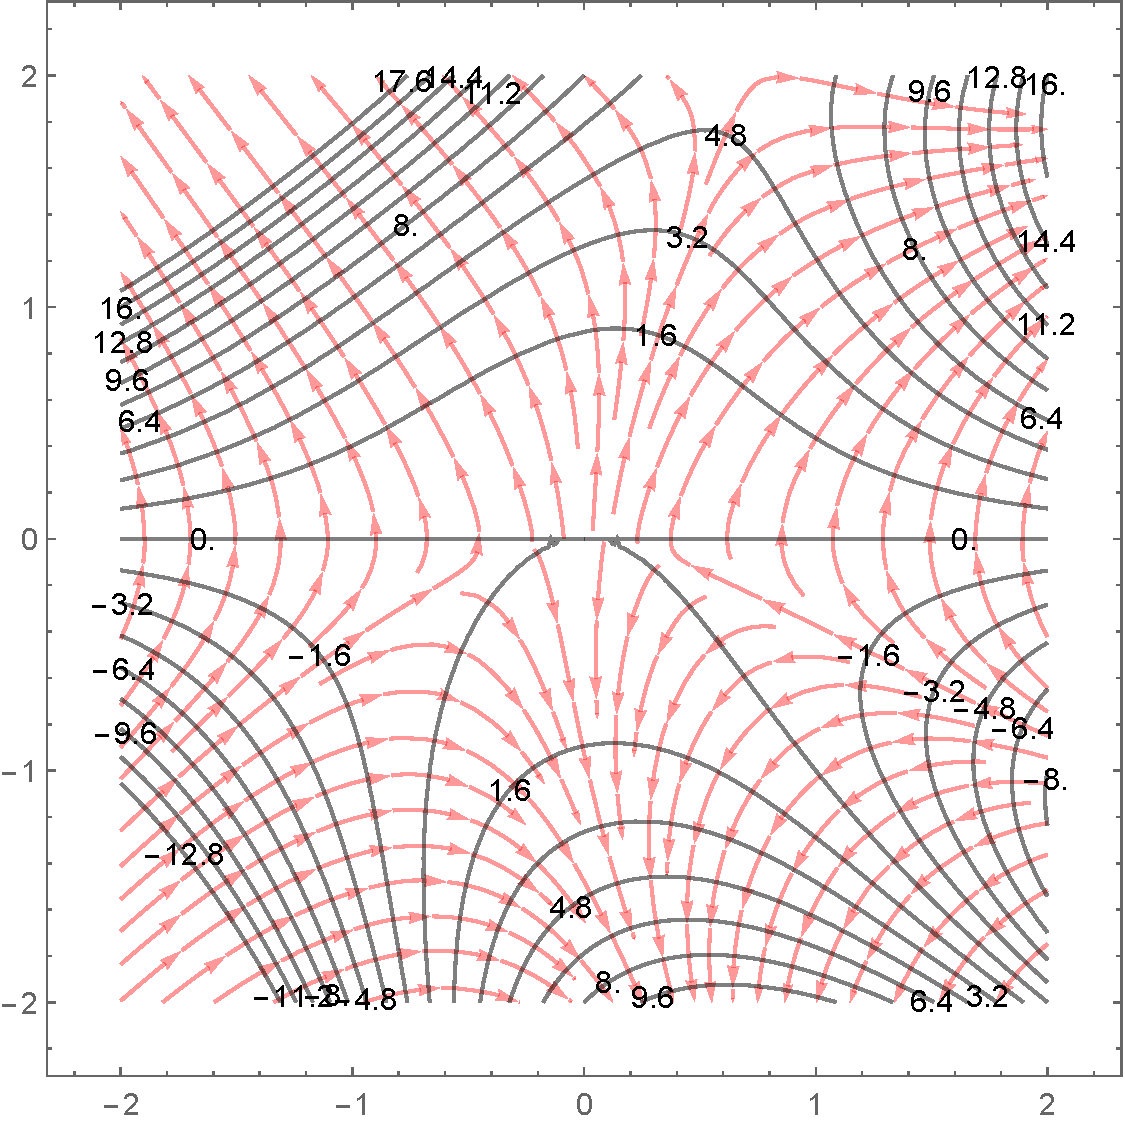
\includegraphics[width=0.7\linewidth]{images/ex4}
		\label{fig:ex4}
	\end{figure}
	
	\begin{figure}[H]
		\centering
		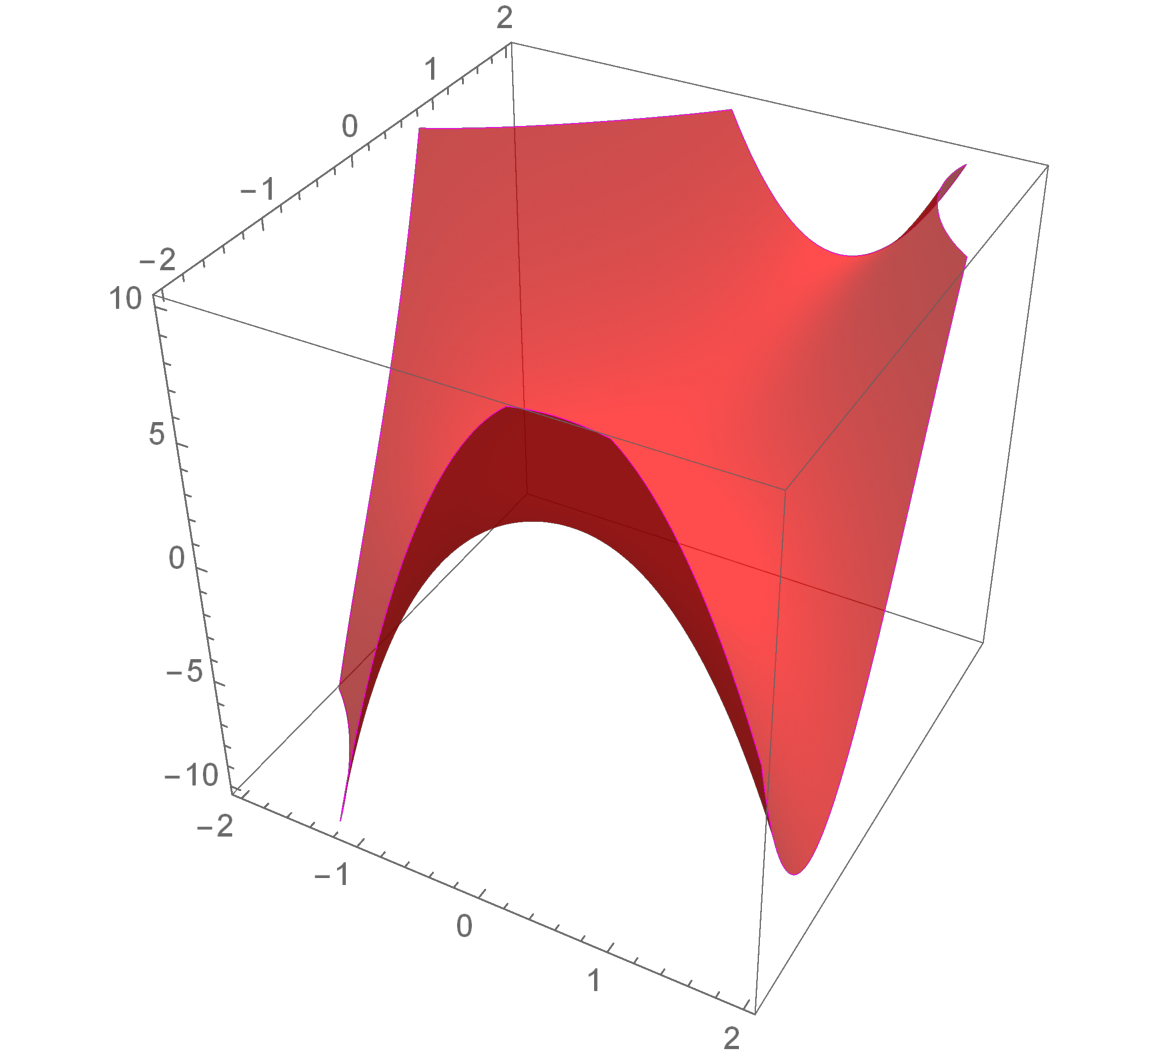
\includegraphics[width=.5\linewidth]{images/ex4_3d1}
		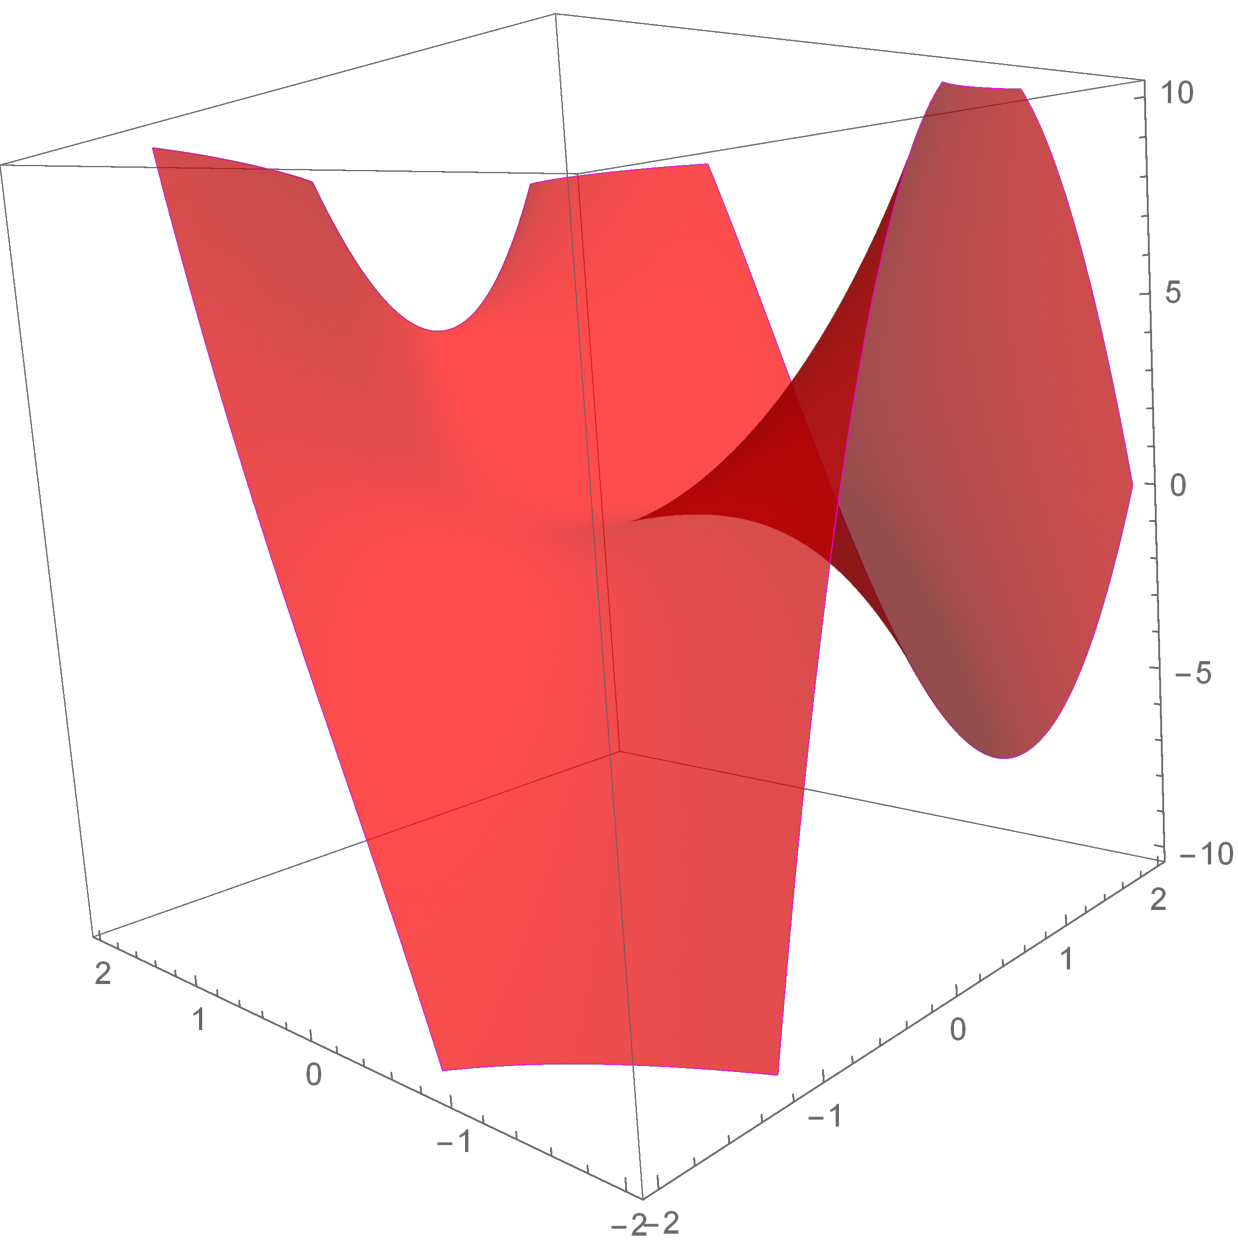
\includegraphics[width=.4\linewidth]{images/ex4_3d2}
	\end{figure}
	\subsection{Exercício 1}
	
	Campo vetorial dado
	
	\begin{equation}
		\force (x,y)=(2x+3y)\vvi+(3x+2y)\vvj
	\end{equation}
	
	As funções $P$ e $Q$ dependentes de $x$ e $y$, nesse caso, são dadas por
	$$
		\begin{cases}
			P(x,y)=2x+3y\\	
			Q(x,y)=3x+2y
		\end{cases}
	$$
	
	A seguinte condição de que
	\begin{equation}
		\dfrac{\partial P}{\partial y}=\dfrac{\partial Q}{\partial x}
	\end{equation}
	
	é satisfeita. Logo existe uma função potencial $f(x,y)$ definida em $\mathbb{R}$. Ao definir que $\partial f/\partial x=P(x,y)$ e $\partial f/\partial y=Q(x,y)$, temos que
	\begin{eqnarray}
		f(x,y)&=&\int P(x,y)\,dx\Rightarrow\\
		&=&\int(2x+3y)\,dx\Rightarrow\\
		\therefore f(x,y)&=&x^{2}+3xy+\xi(y)\label{eq:f1}
	\end{eqnarray}
	
	Igualando a derivada da $f$ anterior com relação a $y$ a $Q(x,y)$, vem
	\begin{eqnarray}
		3x+\xi'(y)&=&3x+2y\Rightarrow\\
		\Rightarrow\xi'(y)&=&2y
	\end{eqnarray}

	Para obter $\xi(y)$, basta integrar a equação anterior, de modo que
	
	\begin{eqnarray}
		\int\dfrac{\xi(y)}{dy}dy&=&\int 2y\,dy\\
		&=&y^{2}
	\end{eqnarray}
	
	Retornando em \eqref{eq:f1} e substituindo $\xi$, vem:
	
	\begin{equation}
		f(x,y)=x^{2}+3xy+y^{2}
	\end{equation}
	
	Agora que temos tanto o campo vetorial quanto a função potencial com os contornos ortogonais ao campo é possível aplicar o \textit{software}. No \textit{Mathematica}, para plotar o campo de vetores, basta usar o \texttt{StreamPlot} (Obs: O \texttt{VectorPlot} também é uma opção no caso).
	
	Para o item estudado ficaria
	
	\begin{center} 			 \texttt{field1 = StreamPlot[\{2x+3y,3x+2y\},\{x,-2,2\},\{y,-2,2\}]}
	\end{center}

	Para os contornos
	
	\begin{center}
		\texttt{contours1 = ContourPlot[x$^{\texttt{2}}$+3yx+y$^{\texttt{2}}$,\{x,-2,2\},\{y,-2,2\}]}
	\end{center}

	Juntando os dois no \texttt{Show}
	
	\begin{center}
		\texttt{Show[contour1, stream1]}
	\end{center}
	Após dar \texttt{<enter>}, obtemos
	
	\begin{figure}[H]
		\centering
		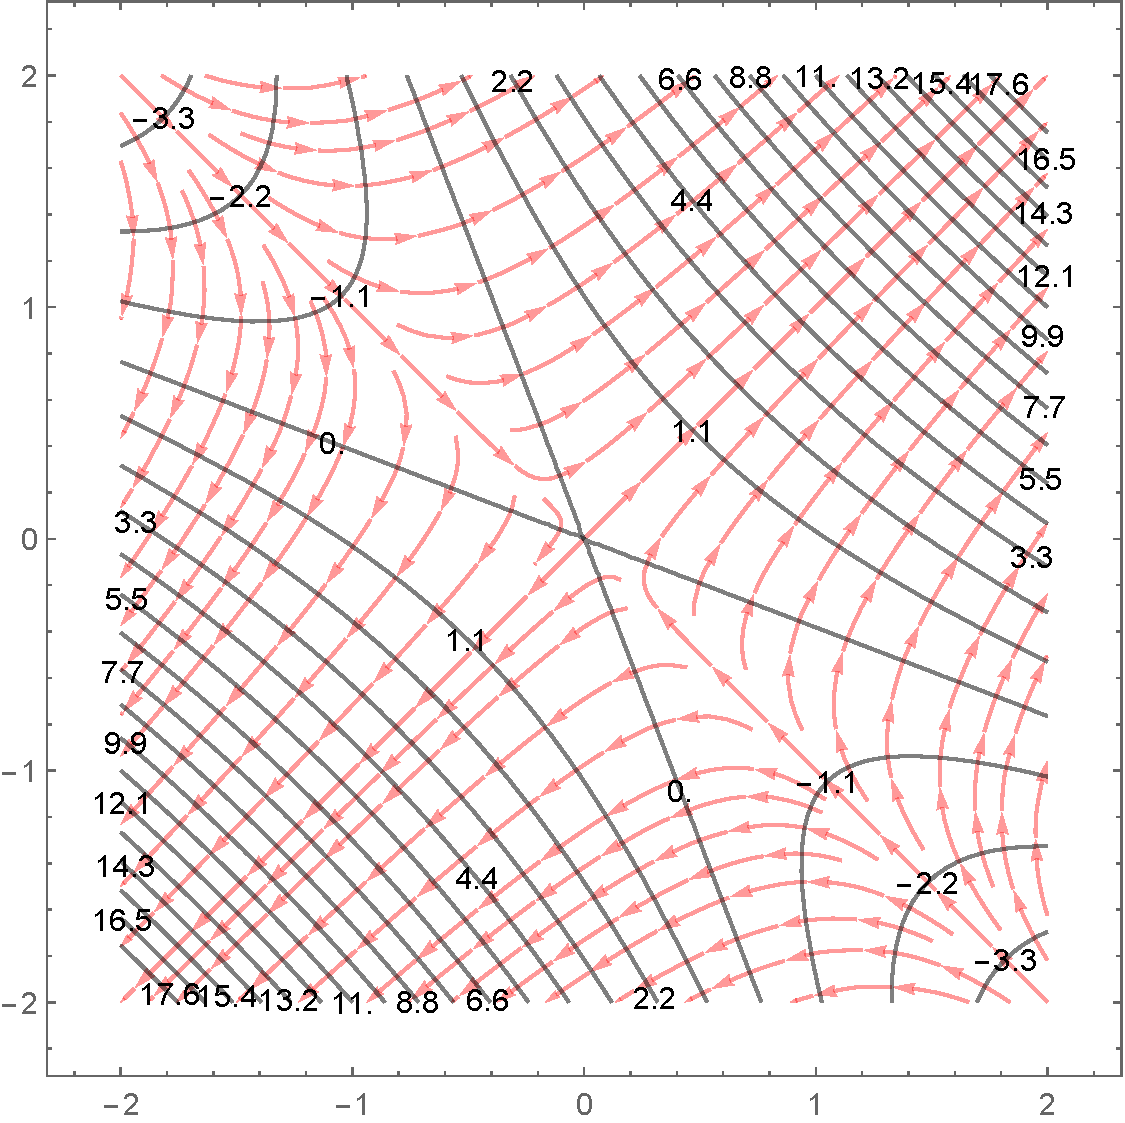
\includegraphics[width=0.7\linewidth]{images/g1}
		\label{fig:g1}
	\end{figure}

	\subsection{Exercício 2}
	
	Campo vetorial
	
	\begin{equation}
		\force (x,y)=(4x-y)\vvi+(6y-x)\vvj
	\end{equation}
	
	Funções $P$ e $Q$
	
	$$
	\begin{cases}
		P(x,y)=4x-y\\
		Q(x,y)=6y-x
	\end{cases}
	$$
	Condição
	\begin{equation}
	\dfrac{\partial P}{\partial y}=\dfrac{\partial Q}{\partial x}=-1 
	\end{equation}
	Função potencial dada a partir de $\partial f/\partial x$
	\begin{eqnarray}
		f(x,y)&=&\int P(x,y)\,dx\\
		&=&2x^{2}-yx+\xi (y)
	\end{eqnarray}
	Estabelecendo a igualdade análoga ao exercício anterior, temos
	\begin{eqnarray}
		\dfrac{\partial f(x,y)}{\partial y}&=&-x+\xi'(y)\\
		6y\cancel{-x}&=&\cancel{-x}+\xi'(y)\\
		\xi(y)&=&6y
	\end{eqnarray}
	
	Logo
	
	\begin{equation}
		f(x,y)=2x^{2}-yx+3y^{2}
	\end{equation}
	
	No \textit{Mathematica}, ao juntar o campo com os contornos, temos
	
	\begin{figure}[H]
		\centering
		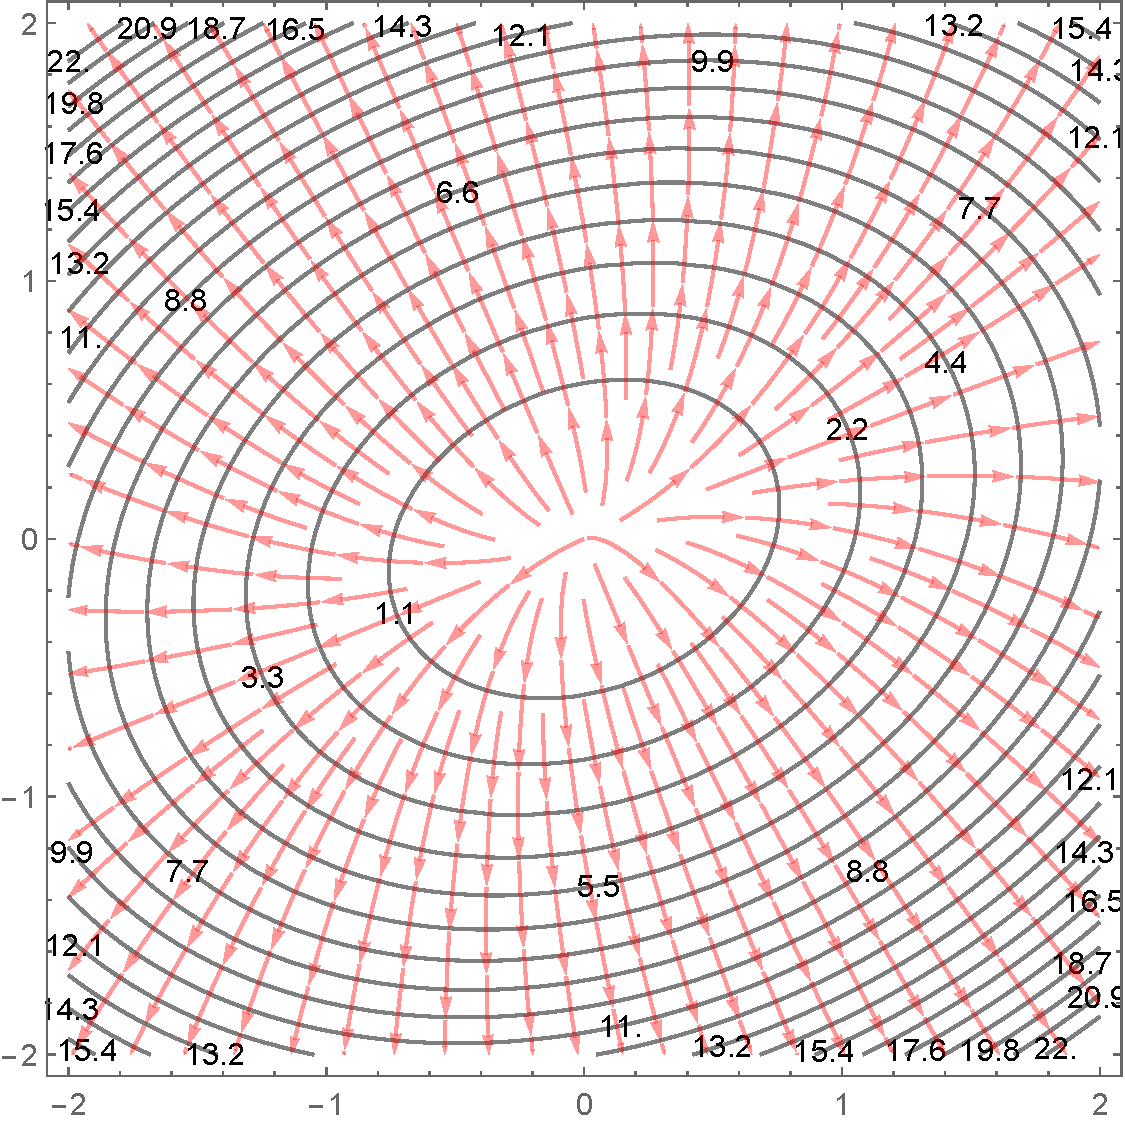
\includegraphics[width=0.7\linewidth]{images/g2}
		\label{fig:g2}
	\end{figure}
	
	\subsection{Exercício 3}
	
	Partindo do campo vetorial definido por
	\begin{equation}
		\force (x,y)=(3x^{2}+2y^{2})\vvi+(4xy+6y^{2})\vvj
	\end{equation}
	
	Tomando $P$ e $Q$ como anteriormente verifica-se que se considerarmos $f(x,y)$ a partir de $\partial f/\partial x$ a função $\xi(y)$ que deveria depender somente de $y$ terá um termo dependente de $x$. Portanto, uma manobra cabível é considerar $\partial f/\partial y=Q(x,y)$ e obter uma função arbitrária agora dependente de $x$ como segue	
	\begin{eqnarray}
		f(x,y)&=&\int Q(x,y)\,dy\\
		&=&2xy^{2}+2y^{3}+\xi(x)
	\end{eqnarray}
	Consequentemente
	\begin{eqnarray}
		2y^{2}+\xi'(x)&=&3x^{2}+2y^{2}
	\end{eqnarray}
	Simplificando
	\begin{eqnarray}
	\bcancel{2y^{2}}+\xi'(x)&=&3x^{2}+\bcancel{2y^{2}}
	\end{eqnarray}
	Então após integrar chega-se que $\xi(x)=x^{3}$ e $f(x,y)$ será
	
	\begin{equation}
		f(x,y)=2xy^{2}+2y^{3}+x^{3}
	\end{equation}
	
	A representação gráfica será
	
	\begin{figure}[H]
		\centering
		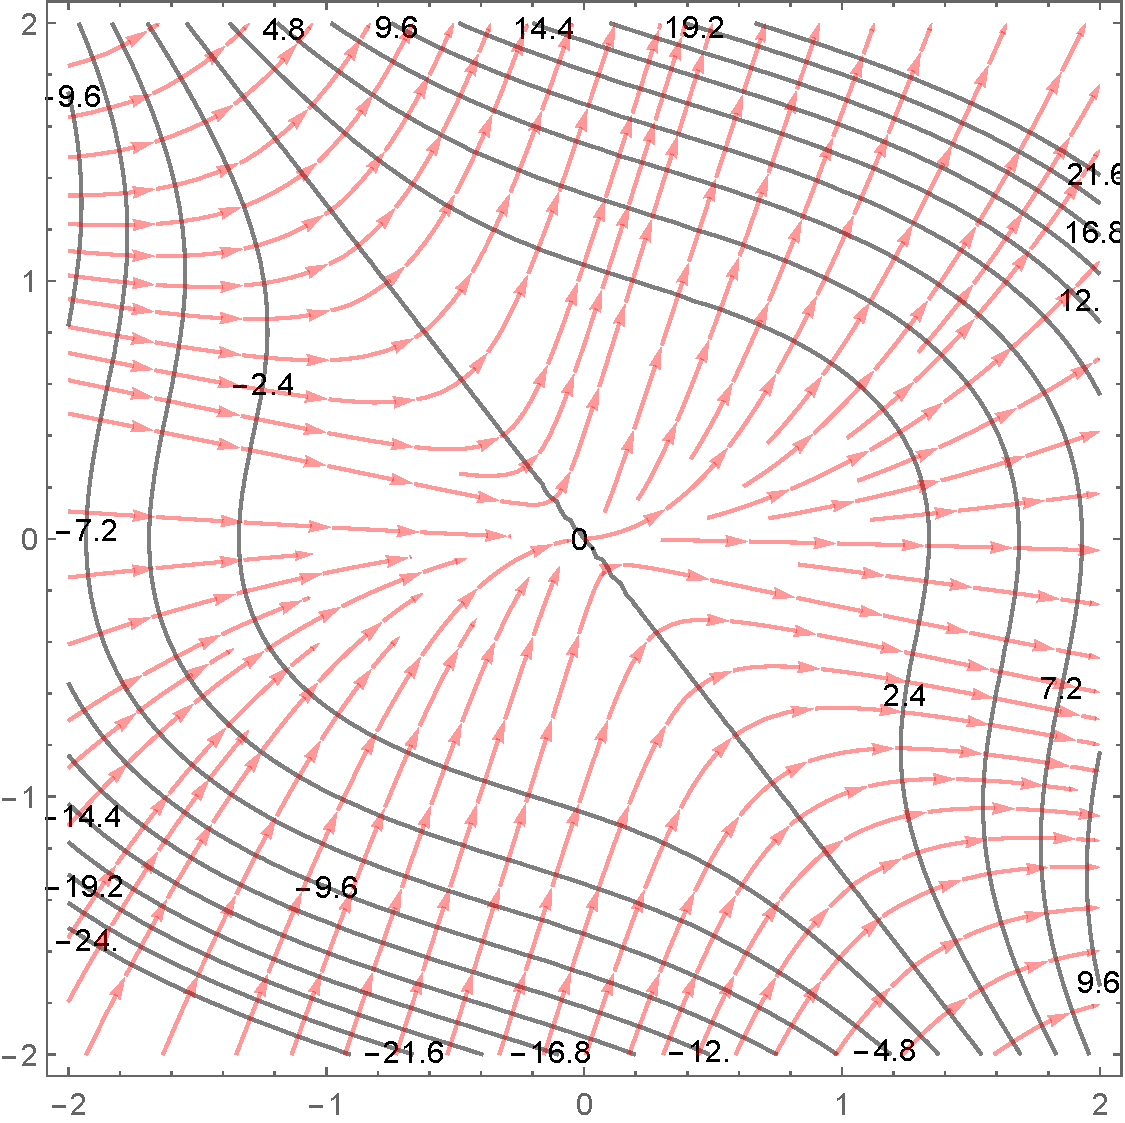
\includegraphics[width=0.7\linewidth]{images/g3}
		\label{fig:g3}
	\end{figure}
	
	\subsection{Exercício 9}
	
	Nesse exercício considerando os artifícios apresentados no Exemplo 3, para o campo vetorial dado por
	\begin{equation}
		\force (x,y)=(3^{2}y^{3}+y^{4})\vvi+(3x^{3}y^{2}+y^{4}+4xy^{3})\vvj
	\end{equation}
	
	Sabendo que o campo é conservativo e considerando a seguinte integral curvilínea que será independente do trajeto
	\begin{equation}
		f(x_{1},y_{1})=\int\limits_{A}^{B}\force\cdot\textbf{T}\,ds
	\end{equation}
	
	podemos escrever
	
	\begin{eqnarray}
		f(x_{1},y_{1})&=&\int\limits_{A}^{B}(3^{2}y^{3}+y^{4})\,dx+(3x^{3}y^{2}+y^{4}+4xy^{3})\,dy
	\end{eqnarray}
	
	seja $C$ a trajetória retilínea do ponto $A=(0,0)$ ao ponto $B=(x_{1},y_{1})$ assumindo a parametrização $x=x_{1}(t)$, $y=y_{1}(t)$ para $0\leq t\leq 1$, então
	
	\begin{eqnarray}
	f(x_{1},y_{1})&=&\int\limits_{A}^{B}(3^{2}y^{3}+y^{4})\,dx+(3x^{3}y^{2}+y^{4}+4xy^{3})\,dy\\
	&=&\int\limits_{0}^{1}[(3x_{1}^{2}y_{1}^{3}t^{5})(x_{1}\,dt)+(3x_{1}^{3}y_{1}^{2}t^{5}+y_{1}^{4}t^{4}+4x_{1}y_{1}^{4}t^{4})(y_{1}\,dt)]
	\end{eqnarray}
	
	\begin{eqnarray}
		&=&\int\limits_{0}^{1}(\red{3x_{1}^{3}y_{1}^{3}t^{5}}+\blue{x_{1}y_{1}^{4}t^{4}}+\red{3x_{1}^{3}y_{1}^{3}t^{5}}+y_{1}^{5}t^{4}+\blue{4x_{1}y_{1}^{4}t^{4}})\,dt\\
		&=&\left[x_{1}^{3}y_{1}^{3}t^{6}+x_{1}y_{1}^{4}t^{5}+\dfrac{y_{1}^{5}}{5}t^{5}\right]_{0}^{1}\\
		f(x_{1},y_{1})&=&x_{1}^{3}y_{1}^{3}+x_{1}y_{1}^{4}+\dfrac{y_{1}^{5}}{5}
	\end{eqnarray}
	
	Fazendo as verificações, temos
	\begin{eqnarray}
		\dfrac{\partial f(x,y)}{\partial x}&=&3x^{2}y^{3}+y^{4}\\
		\dfrac{\partial f(x,y)}{\partial y}&=&3y^{2}x^{3}+4xy^{3}+y^{4}
	\end{eqnarray}
	
	logo, há concordância entre o obtido e as componentes escalares de $\force$.
	
	Graficamente, chegamos
	
	\begin{figure}[H]
		\centering
		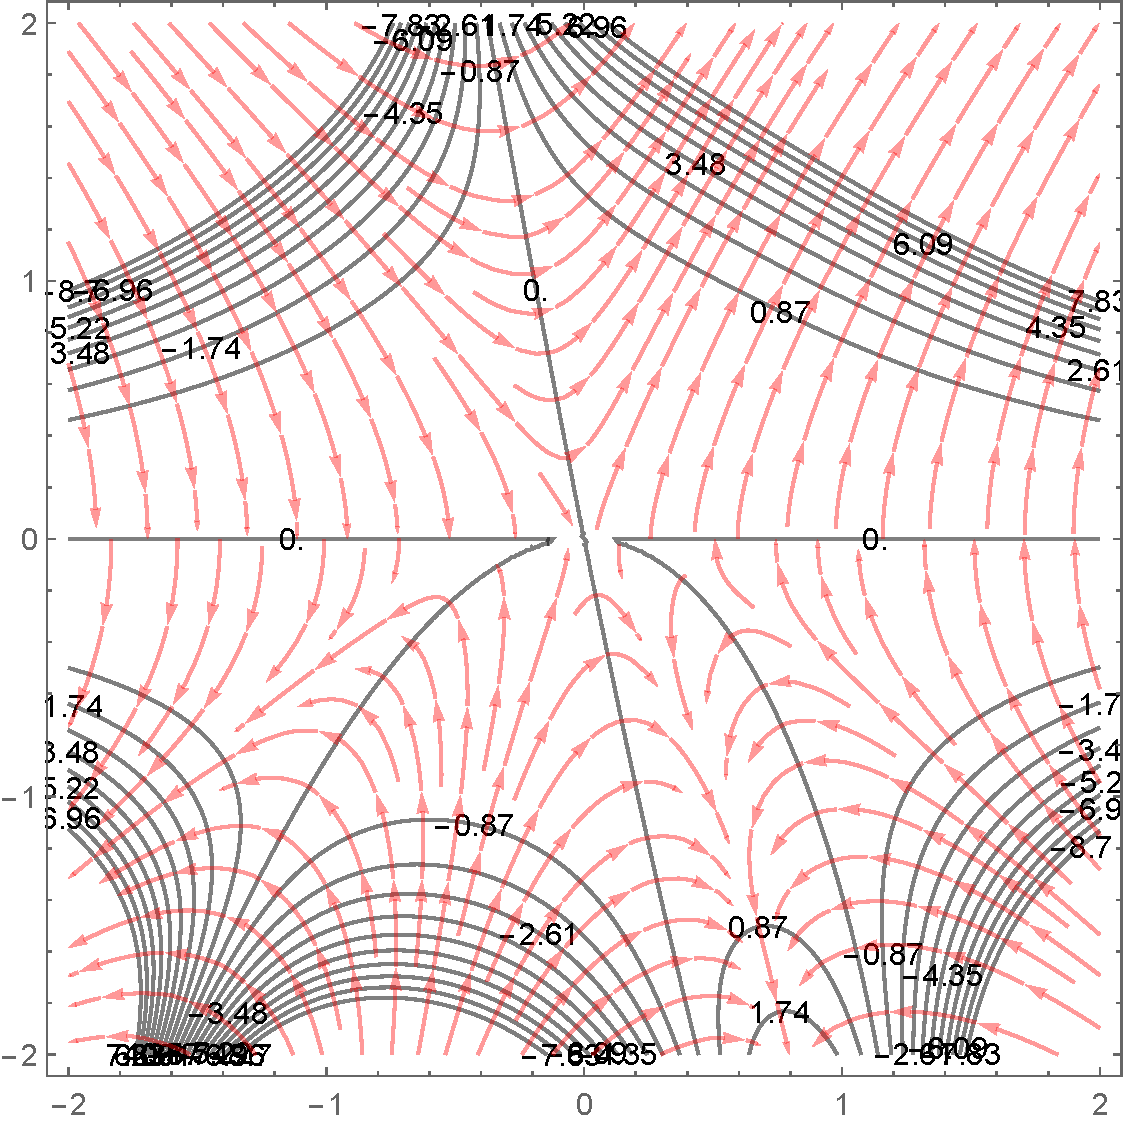
\includegraphics[width=0.7\linewidth]{images/g15}
		\label{fig:g15}
	\end{figure}

	Ao aplicar o \texttt{ContourPlot3D} para ps contornos, chegamos na seguite configuração de superfície
	
	\begin{figure}[H]
		\centering
		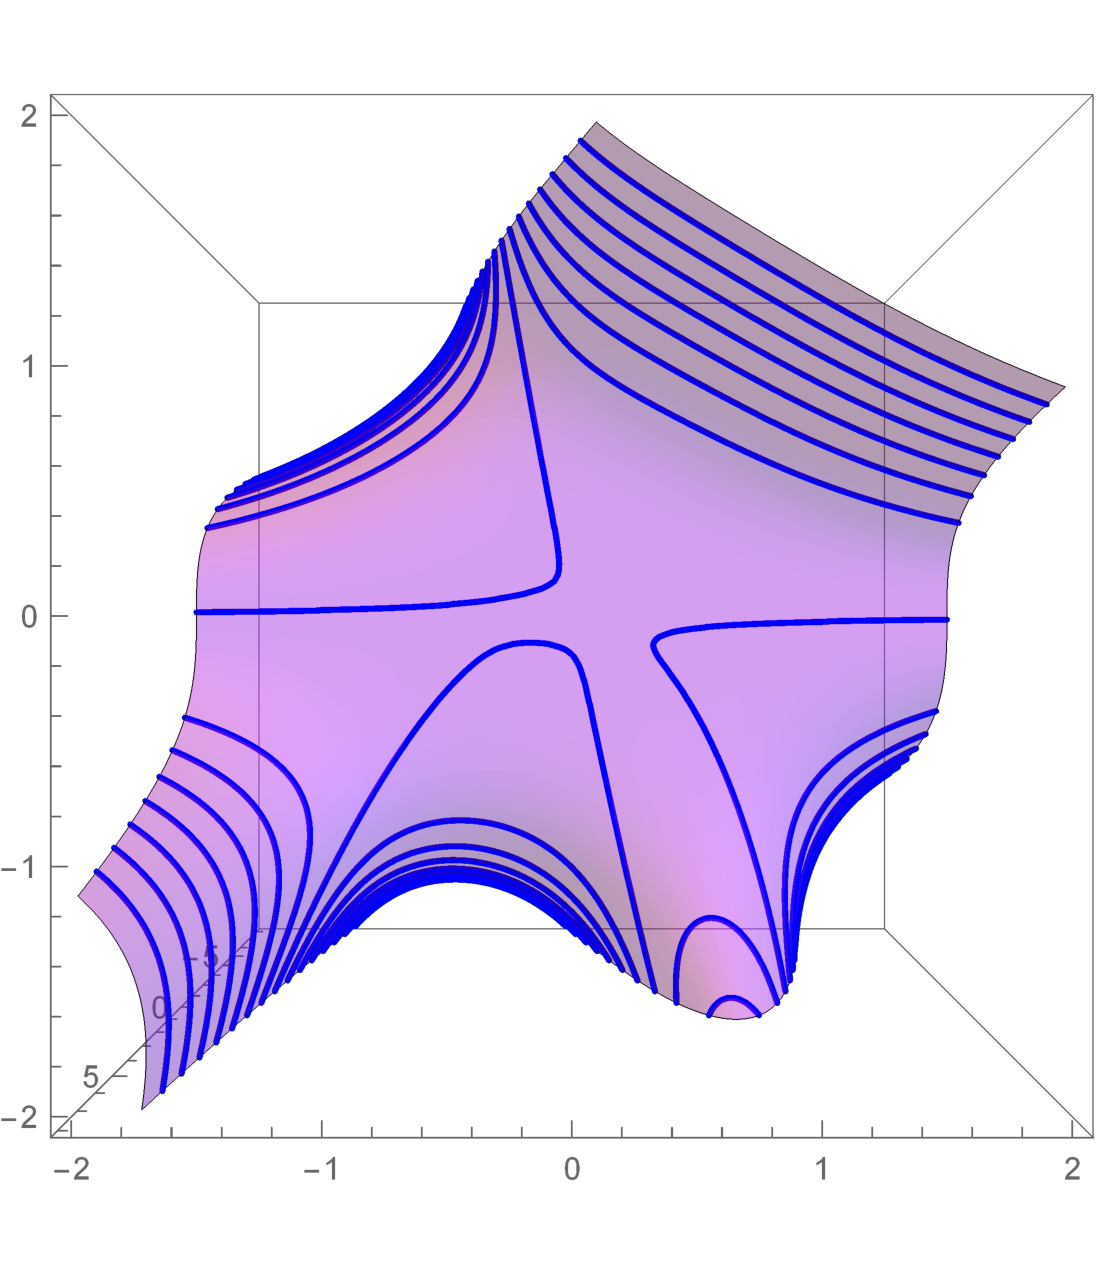
\includegraphics[width=0.6\linewidth]{images/g153d1}
		\caption{Vista superior}
	\end{figure}

	\begin{figure}[H]
		\centering
		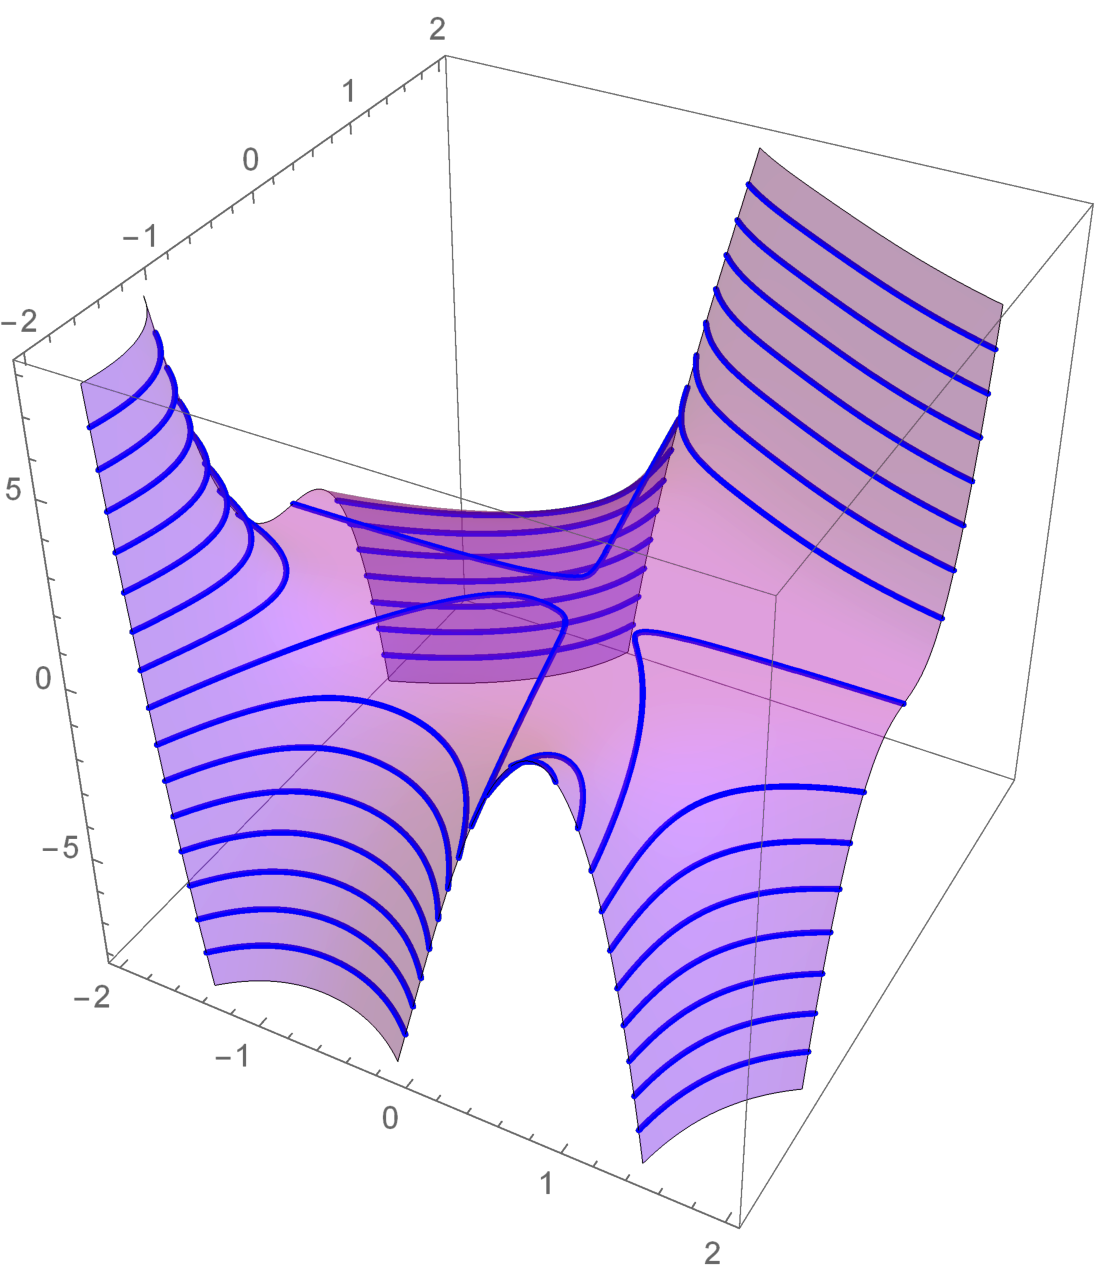
\includegraphics[width=0.6\linewidth]{images/g153d2}
		\caption{Vista padrão}
	\end{figure}
	
	\subsection{Exercício 26}
	
	Campo vetorial de quadrados inversos
	\begin{equation}
		\force (x,y)=\dfrac{-y\vvi+x\vvj}{x^{2}+y^{2}}
	\end{equation}
	
	O valor obtido na integral curvilínea 
	\begin{equation}
		\int\force\,d\textbf{r}
	\end{equation}
	
	pode ser interpretado como o trabalho da partícula ao longo do campo vetorial apresentado. Porém, nesse caso é interessante aplicar a parametrização já que a trajetória descrita é a de uma circunferência. Sendo assim, a posição de uma partícula expressa como função do deslocamento angular pode ser dado por
	\begin{equation}
		\textbf{r}(t)=\cos t\,\vvi+\sin t\,\vvj
	\end{equation}
	
	\begin{figure}[H]
		\centering
		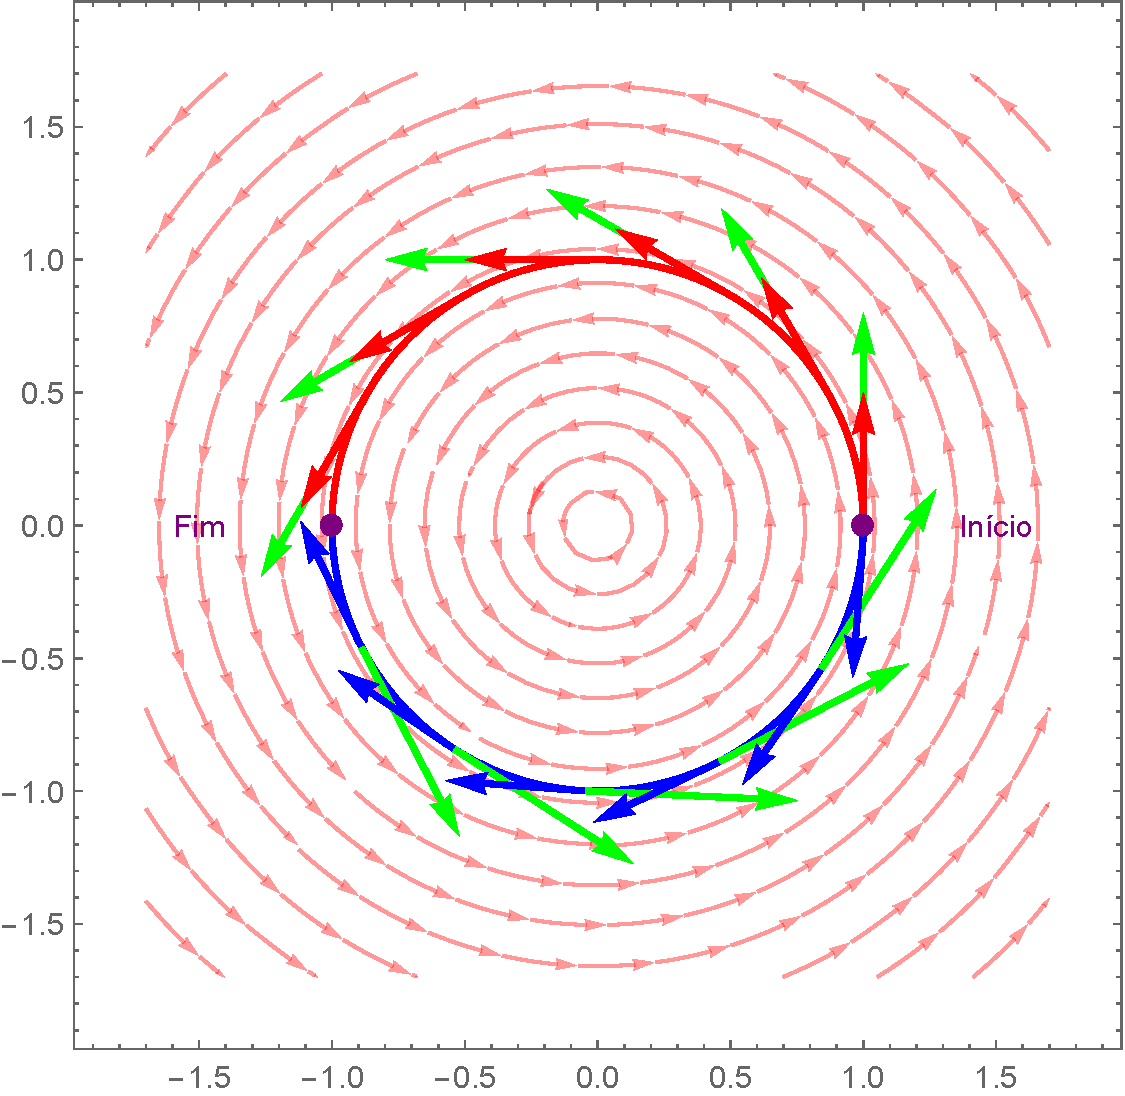
\includegraphics[width=0.7\linewidth]{images/g26}
		\label{fig:g26}
	\end{figure}

	Para obter o elemento $d\textbf{r}$ da integral curvilínea, basta derivar a função da posição, logo
	\begin{eqnarray}
		\dfrac{d\textbf{r}}{dt}&=&-\sin t\,\vvi+\cos t\,\vvj\\
		d\textbf{r}&=&-\sin t\,dt\,\vvi+\cos t\,dt\,\vvj
	\end{eqnarray}
	
	Após substituir as componentes de \textbf{r} em \force, vem
	\begin{eqnarray}
		\force(t)&=&\dfrac{-\sin t\,\vvi+\cos t\,\vvj}{\cos^{2}t+\sin^{2}t}\Rightarrow\\
		\force(t)&=&-\sin t\,\vvi+\cos t\,\vvj
	\end{eqnarray}
	
	A integração no arco superior com $0\leq t\leq\pi$ será
	\begin{eqnarray}
		W&=&\int\limits_{0}^{\pi}\force(t)\,d\textbf{r}(t)\\
		&=&\int\limits_{0}^{\pi}\sin^{2}t\,dt+\cos^{2}t\,dt\\
		&=&\int\limits_{0}^{\pi}dt\\
		t\,\bigg|_{0}^{\pi}&=&\pi
	\end{eqnarray}
	
	Se tratarmos o mesmo início e fim da trajetória anterior mas pelo arco de baixo, teremos $0\leq t\leq -\pi$ e a integral assumirá	
	\begin{eqnarray}
		W&=&\int\limits_{0}^{-\pi}\,dt\\
		t\,\bigg|_{0}^{-\pi}&=&-\pi\\
	\end{eqnarray}
	
	Com base na análise dos valores obtidos para as integrais curvilíneas, vê-se que o trabalho exercido pelas forças de campo é positivo para o arco superior. O resultado é coerente tendo em vista que as linhas do campo vetorial possuem mesma direção e sentido com o deslocamento $dr$. Dessa forma, o produto ponto entre os vetores	
	\begin{equation}
		\force\,d\textbf{r}=||\force||\,||d\textbf{r}||\cos\theta
	\end{equation}
	
	com $\theta=0^{\circ}$ ao longo de todo o percurso ocasionará num trabalho positivo. Em contrapartida, ao partir do início mostrado na figura e percorrer a trajetória circular no sentido horário, há contraposição entre o deslocamento e as linhas de campo. Como $\theta=180^{\circ}$, $W<0$.
	
	Quando se usa a definição de campos conservativos e funções potenciais vistas no livro, conclui-se que existe $\force=\nabla f$ já que o trabalho ao longo do percurso independe da trajetória no exercício estudado. Entretanto, partindo-se das derivadas parciais $\partial P/\partial y$ e $\partial Q/\partial x$, verifica-se que
	\begin{equation}
		\dfrac{\partial P}{\partial y}\neq\dfrac{\partial Q}{\partial x}
	\end{equation} 
	então o campo não é conservativo.
	
	
	
\end{document}